\documentclass[12pt,a4paper]{scrartcl}
\usepackage[utf8]{inputenc}
\usepackage[english]{babel}
\usepackage{amsmath}
\usepackage{amsfonts}
\usepackage{amssymb}
\usepackage[T1]{fontenc}
\usepackage{ae,aecompl}
\usepackage{graphicx}
\usepackage{wrapfig} 
%\usepackage{subfig} % see here: https://tex.stackexchange.com/questions/13625/subcaption-vs-subfig-best-package-for-referencing-a-subfigure
\usepackage{subcaption} % support subplots
\usepackage{caption}
\usepackage{pdfpages}
\usepackage{geometry}
 \geometry{
 a4paper,
 total={160mm,240mm},
 left=25mm,
 top=30mm,
 }

\usepackage[parfill]{parskip} % Activate to begin paragraphs with an empty line rather than an indent

% FONT
\renewcommand{\familydefault}{\sfdefault}
\graphicspath{ {_illustrations/} }

\usepackage[%
%    %%% general options
%    pdftex=true,      %% sets up hyperref for use with the pdftex program
%    %plainpages=false, %% set it to false, if pdflatex complains: ``destination with same identifier already exists''
%    %
%    %%% extension options
%    backref,      %% adds a backlink text to the end of each item in the bibliography
%    pagebackref=false, %% if true, creates backward references as a list of page numbers in the bibliography
	hidelinks,
    colorlinks=false,   %% turn on colored links (true is better for on-screen reading, false is better for printout versions)
%    linkcolor=blue,
%    citecolor=blue,    
%    %%% PDF-specific display options
    bookmarks=true,          %% if true, generate PDF bookmarks (requires two passes of pdflatex)
    bookmarksopen=true     %% if true, show all PDF bookmarks expanded
%    bookmarksnumbered=false, %% if true, add the section numbers to the bookmarks
%    %pdfstartpage={1},        %% determines, on which page the PDF file is opened
%    pdfpagemode=None         %% None, UseOutlines (=show bookmarks), UseThumbs (show thumbnails), FullScreen
  ]{hyperref}


%%% title
\title{Labeling Roads in Satellite Imagery of Rural Areas}
\subtitle{A Guide to Digitizing Roads with QGIS}
%%% author(s)
\author{Harald Hentschke, Erik Seiert}

%%% date
\date{Berlin and Tübingen, \today{}}

\begin{document}
\maketitle
\newpage

\tableofcontents
\newpage

\section{Background} 
The origins of this manual date back to the summer of 2018, when three Data Scientists-to-be (Lisa He\ss e, Krian Prakash, Harald Hentschke) developed a deep learning model for the detection of roads in satellite imagery as their portfolio project for \href{https://www.datascienceretreat.com/}{Data Science Retreat} in Berlin. Version~1 of the manual, written by Harald Hentschke, detailed the whole procedure as accomplished with Google Earth, including the merging and correction of pre-existing labels from different sources, defining naming conventions, etc.

Upon continuation of the project during a Microsoft-sponsored AI for Earth grant (May 2019 -- April 2020), Erik Seiert wrote a manual for digitizing roads using QGIS, which has several advantages over Google Earth. 

The present manual is an amalgam of both: it details the procedure of producing high-quality road labels for our purposes from beginning to end, including sighting and correction of existing labels, and exact definitions of naming conventions (which may appear as an unnecessary detail, but is in fact quite important for smooth downstream data processing).

Material which is vital only initially or likely to be used as a reference (installation of software, types of data) is placed at the end of the manual.

Contact: \url{hhntschk@gmail.com}

\section{Definitions/abbreviations}
\begin{itemize}
	\item \textbf{Area of interest (AOI):} a region in which roads shall be labeled, for example, 50 by 50 km squares in Borneo as shown in Fig~\ref{fig:aoi}. An AOI is at least as large as a single satellite image, but otherwise its size is deliberately not exactly defined.
	\item \textbf{Sub-area of interest (subAOI):} the part of an AOI that has been completely labeled, or is in the process of being completely labeled, and is marked as such by a polygon that encloses it. \textbf{Delineating labeled areas in this way is the basis of a systematic labeling approach that avoids redundancy and loss of data}.
	\item GE: Google Earth (see Section~\ref{sec:software})
	\item QGIS: see Section~\ref{sec:software}
	\item OSM: Open Street Maps
\end{itemize}

\begin{figure}
	% \centering
	\begin{subfigure}{0.46\textwidth}
		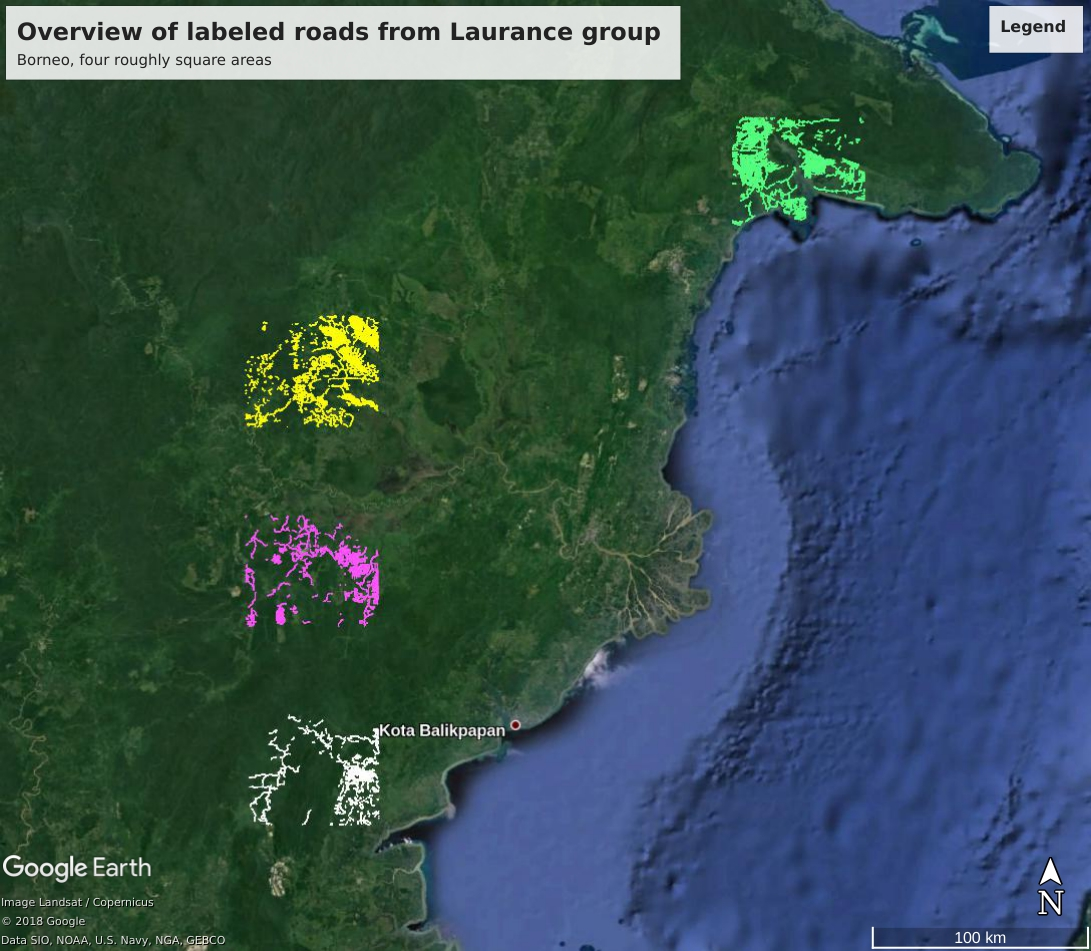
\includegraphics[width=0.88\linewidth]{GE_overview_areas_Borneo.jpg}
	\end{subfigure} 
	\begin{subfigure}{0.5\textwidth}
		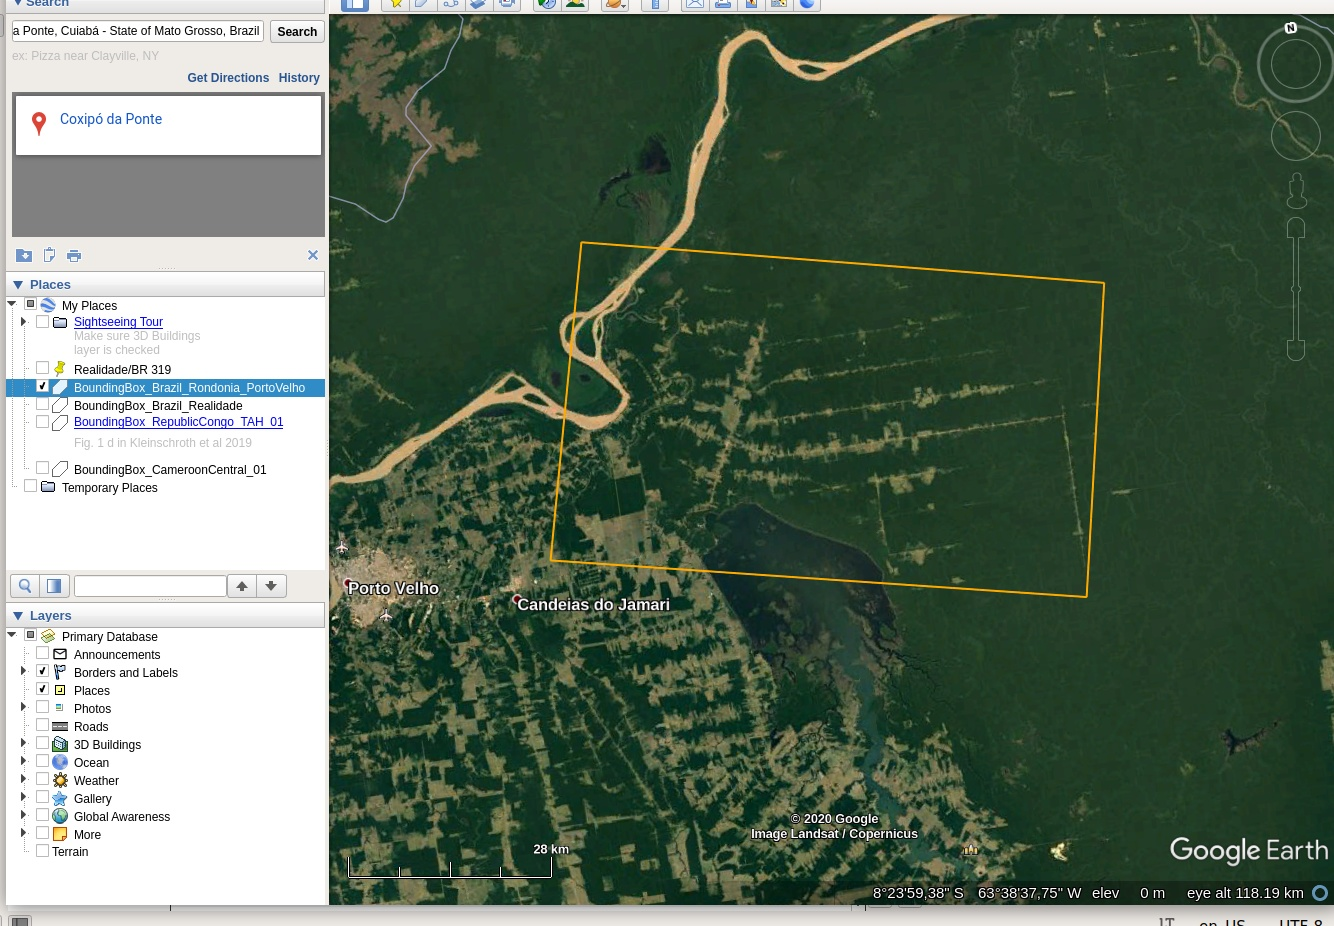
\includegraphics[width=0.99\linewidth]{Screenshot_AOI_example.jpg}
	\end{subfigure} 
	\caption{Left, four areas of interest (AOI) in Borneo, easily discernible via their labels provided by the Global Road Map Initiative. Right, an AOI as defined via a manually drawn polygon in Google Earth. Note it being listed in the 'Places' tab on the left ('BoundingBox\_Brazil\_Rondonia\_PortoVelho'). This polygon has to be exported into kml or kmz format and can then be used by our code for a programmatic retrieval of satellte imagery.}
	\label{fig:aoi}
\end{figure}

\section{Required software}
\label{sec:software}
\begin{itemize}
	\item Google Earth (GE), the ubiquitously known 3D geoviewer. Its installation on common operating systems is straightforward and therefore not explained here.
	\item QGIS, a Geographic Information System, freely available. QGIS bundles many tools in one program to allow a complete workflow from initial data visualisation over complex analysis to complete maps. It is our our main workhorse. The installation of QGIS is a bit involved, see Section~\ref{sec:qgis_install}.
\end{itemize}
	

\section{Workflow: Overview}
The list below outlines the workflow for labeling roads in a new AOI. The initial steps will of course have to be skipped or adapted if roads have already been labeled in parts of it.
\begin{itemize}
	\item Decide on an AOI, mark it via a polygon (\ref{fig:aoi})
	\item Retrieve satellite images from that AOI
	\item Retrieve Open Street Map (OSM) road labels for the AOI
	\item Set up a new project file in QGIS
	\item Load all satellite images of the AOI into QGIS
	\item Set and scale colors of images
	\item Load OSM road labels
	\item Inspect labels and decide whether they are worth keeping
	\item If labels are worth keeping, prune them to the area covered by satellite imagery, if not, discard them
	\item Define an area in which you are going to label roads and/or correct OSM road labels by drawing a polygon around it (this is the subAOI)
	\item If you retained OSM road labels, correct them first
	\item Label new roads
	\item When done with the subAOI, extend it and continue labeling
	\item When done for the session adjust the polygon such that it encloses an area in which there is a 100 \%  correspondence of roads and labels (no missing labels, no superfluous labels)
    \item Save project file
    \item As soon as a subAOI encloses a full satellite image, export the labels in it so they and the satellite images can be used for training right away
\end{itemize}

\section{Workflow: Step-by-step instructions}
\subsection{Selection of an area of interest (AOI)}
tbc

\subsection{Retrieval of satellite images}
tbc

\subsection{Retrieval of Open Street Map data \& other labels}
\href{https://www.openstreetmap.org/}{Open Street Map} has surprisingly accurate and complete maps of roads in some remote areas. It is therefore definitely worth checking out the maps for the AOI at hand. It is possible to download them from within QGIS, but this may be the topic of a future version of the manual. For now, we'll do this manually. At \url{https://planet.openstreetmap.org/} sites for download are listed. If you are located in Europe/Germany, selection of a relevant subset and download from \url{http://download.geofabrik.de/} works pretty well.

It goes without saying that checking already existing labels for specific regions must come first. From the initial phase of the project, there are labels for the German region of Harz and for Borneo. For Borneo, labels from the Global Road Map Initiative (Sean Sloan, Laurance group) may want to be revisited, although these have issues and may generally be too crude for our purposes. Please talk to Harald for any related questions.

\subsection{Basic set up of a project file}
\label{step2}
If this is the first time you work with QGIS, see Section~\ref{subsec:qgis_adjust}, which describes the installation of plugins and the general setup of QGIS.

Working with QGIS is convenient only with a well-ordered data structure. Of course you can adhere to your own naming conventions, but for the sake of unambiguous communication, the directory and file names below will be assumed throughout the manual. 

For a new AOI to be labeled, create folder
\begin{verbatim}
<path to your datafolder>/labeling_stage
\end{verbatim}
and distribute data in the following subfolders:
\begin{verbatim}
satellite_images
subAOI
labels_OSM
labels
\end{verbatim}


Start QGIS. Set up a project in which the data labeling will take place: click on 'New Empty Project' in the main window or click \textit{Project - New}. 

\subsubsection{Project Properties}
\label{subsec:project_properties}
Open the project properties either by pressing \textit{ctrl + shift + p} or click \textit{Project} and then \textit{Properties}. A window will pop up with menu items/tabs on the left, and edit fields, drop-down lists etc. to the right. 

\begin{itemize}
	\item{General} 
	\begin{itemize}
		\item \textbf{General Settings}: Set the project path to \textit{(path to your datafolder)/labeling\_stage}. Set a project title. Make sure that the "Save Paths" option is \textit{relative}.
		\item \textbf{Measurements}: By default, the calculations ellipsoid should be set to "WGS 84". Leave the default, as it is a widely used reference. Change only if you know what you are doing/ there are problems with display of certain layers. All other options in this rider should be in the metric system to avoid complications.
		\item \textbf{Coordinate Display}: It is recommended to change the option "display coordinates" to decimal degrees which is the same as the google maps display style.
	\end{itemize}
	
	\item{CRS}\\ 
	Change to the menu item "CRS" (Coordinates: datum and system). Here you can check if the Project Coordinate Reference System is also set to WGS 84. If not, you can change it by Filtering/Searching for 4326 which is the EPSG number of the WGS 84 system.
	
	For reference purposes, you can set the Coordinate System to WGS84/ Pseudo Mercator (EPSG: 3857). \textbf{This coordinate system is used by google maps, which you may want to use to double-check locations}.
\end{itemize}

Apply the properties by clicking on Apply or OK.


\subsection{Loading satellite images into QGIS}
\label{step3}
There are multiple ways to load satellite images. The most convenient is to drag and drop images from the 'Project Home' folder as seen in the 'Browser' window into the main window. Alternatively, click \textit{Layer} - \textit{Add Layer} - \textit{Add Raster Layer} - click the \textit{...} button, then choose the satellite image from your Sat Image folder and click \textit{open}

It is highly recommended to load \textbf{all} satellite images of an AOI, or at least groups of adjacent and/or overlapping images. The reason is that then the time-consuming act of pruning OSM road labels (one of the next steps) needs to be done only once (per group of adjacent images). However, be aware that images may overlap, in other words occlude each other partly, a situation which can potentially lead to inadvertently incomplete labels.


\subsubsection{Display, navigation, overview}
The display of the data can be managed in the Layers window (optimally at the left side of the screen). There you can change the order of display by drag \& drop and disable/enable the layers by un/checking the checkbox. \textbf{Hint:} \textit{Right mouse click - Zoom to Layer} allows you to quickly zoom in on the selected layer on the screen.

It is very important to get an overview of the area you are working on. This is not only true for labeling but for all kinds of remote sensing work, so you can avoid mix-ups of landscape features and get a feel for the characteristics of a region.  

You can double check where you are with the coordinate capture plugin (described briefly in Chapter \ref{coordcap}).
Try and get get the coordinates of a point on the map e.g. a city or village or a prominent landscape feature. 
Copy those coordinates in decimal degrees (described in Chapter \ref{step2}) and paste them in google maps for example. \textbf{Hint:} Be sure to switch the order of the numbers, because QGIS shows the decimal degree coordinates in the order of \textit{Eastings and Northings} while google maps shows them in the order of \textit{Northings and Eastings}.

\subsubsection{Satellite band combinations}
A good way to extract relevant information from satellite imagery is to change the order of image bands.
% In Chapter \ref{rastabands} the concept of bands is illustrated and in Chapter \ref{scpprep} we prepared them for easy manipulation. 
% Because, with the scp plugin installed it is just a matter of a few clicks: \\
% Find the drop down field named "\textit{RGB =        }" in the main window and try a few band combinations.  
% You will see the color of the satellite image changing immediately.\\

I find, for road detection, combining Near Infrared, Blue and Red gives a good contrast (For planetscope this should be 4 - 1 - 3).
Plants like crops will be bright red, water bodies nearly black, forests will also be quite dark, dry fields will be blueish and streets/ buildings and bare soil/ sand will be bright blue.\\

DETAILED INSTRUCTIONS TO COME (PENDING SOLUTION OF SCP PROBLEM)

\subsubsection{Loading, checking, and pruning OSM road labels (and other labels)}
OSM label files usually comprise large geographic areas, so if they turn out to be useful we need to prune them to the area covered by the satellite images of the AOI.

\begin{enumerate}
	\item Load the OSM labels. Labels can be loaded in manners similar to those for images -- drag \& drop or via the Layer menu (labels should be defined as vector layers).
	\item Inspect the label quality. If the labels don't trace the roads very well, delete the layer, and skip the remaining steps in this section. If a \textit{sizeable} amount of labels does trace the roads well, similar to how you would yourself label them, and if you are sure that correcting whichever imperfections these labels have is a substantial time saver over labeling the roads from scratch, continue.
	\item Using one of QGIS' selection tools, select the road labels you'd like to keep (see Figure~\ref{fig:mark_osm_label} for details). No need to be super-precise, road labels protruding beyond the area covered by the satellite images  will be cut off programmatically further down the computational road.	Click Edit-Copy Features (or hit Ctrl-C) and then Edit-Paste Features As (nope, Ctrl-V won't do the trick) and select New Vector layer. In the window that pops up, \textbf{select geojson as format. This is the only currently confirmed format which supports the steps further below}. To the right of the edit field for the file name, click on the three dots to select a directory in which to save the data (otherwise QGIS may select your home directory and you may have trouble finding the file). Name the file according to the scheme <YYYY\_MM\_DD>\_<AOI>\_OSM, where the date is that of the data retrieval, e.g. 2020\_04\_23\_Brazil\_Rondonia\_PortoVelho\_OSM. The layer name will be identical, leave it at that. Make sure CRS is set correctly (see Section \ref{subsec:project_properties}) and leave all other settings as they are.
	\item In the 'Layers' window, mark the whole set of OSM road labels and delete them - we won't need them anymore.
	\item Mark the set of retained labels and go to the Layer Styling tab/window. There, set the width and color to eye-friendly values. This is now our reservoir of labeled roads which we need not label ourselves, but may have to correct.
\end{enumerate}

\begin{figure}
	% \centering
	\begin{subfigure}{0.49\textwidth}
		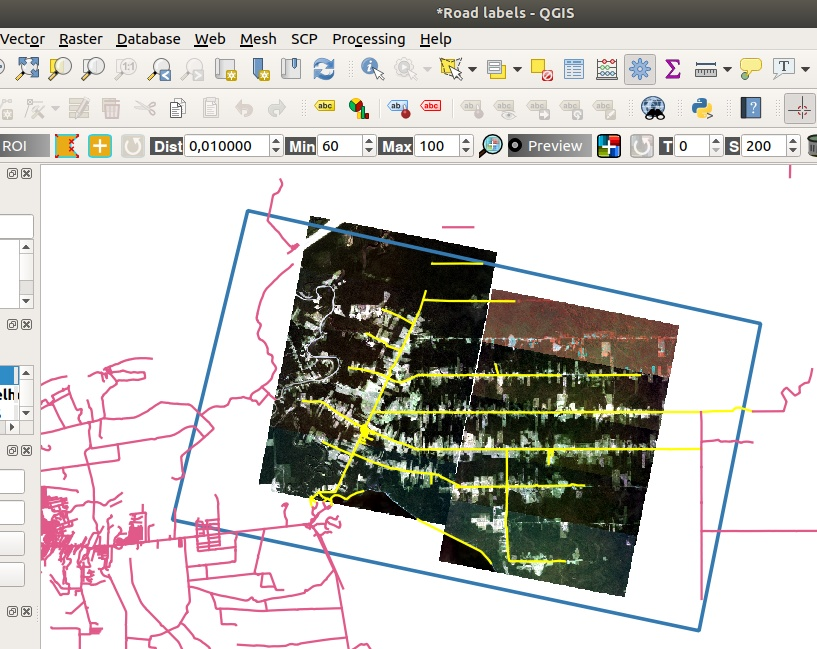
\includegraphics[width=0.99\linewidth]{marking_OSM_labels01.jpg}
	\end{subfigure} 
	\begin{subfigure}{0.49\textwidth}
		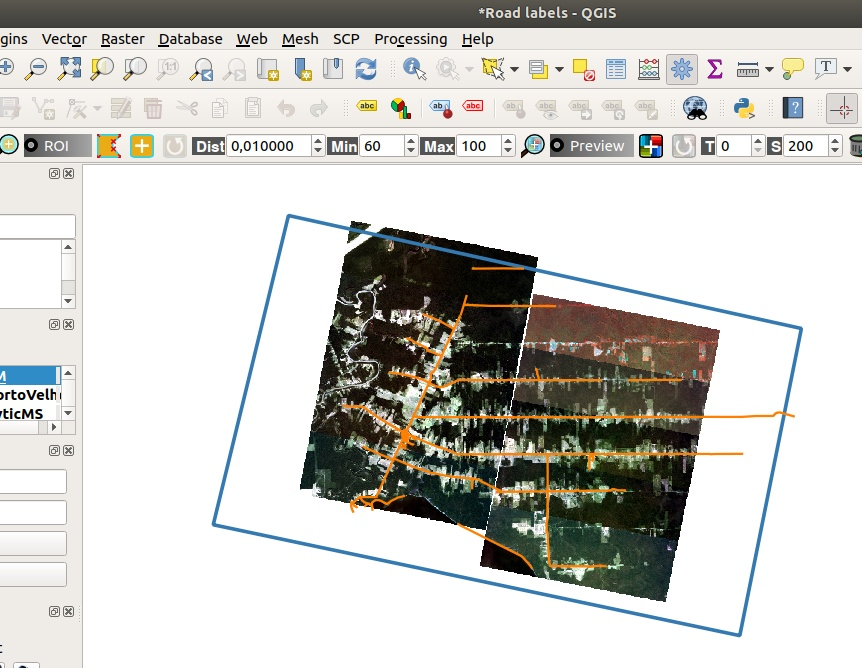
\includegraphics[width=0.99\linewidth]{marking_OSM_labels02.jpg}
	\end{subfigure} 
	\caption{Left, satellite images of one AOI (blue rectangle) with OSM road labels overlaid. The images are arranged in two 'columns' of five images each. The labels coursing within the satellite images have been selected with QGIS' selection tool (the yellow symbol below the 'p' in 'Help') and are marked in yellow. All other labels appear in magenta. Right, the same AOI after the labels to be kept have been copied to a new layer and recolored and the other OSM labels have been deleted.}
	\label{fig:mark_osm_label}
\end{figure}


\subsection{Create/update subAOI}
Once again, a subAOI is the area within which the labels are garanteed to be a) complete b) correct. Experience shows that if you as the labeler return to an incompletely labeled scene, you will struggle to know exactly which areas have been completely labeled. To avoid redundant work or incompletely labeled areas, use polygons to mark the subAOI.

\begin{itemize}
	\item Create a new layer in which the polygon will be stored: Click on the \textit{Layer} Menu Item - \textit{Create Layer} - \textit{New Shape File Layer}. A pop-up window appears.
	\item To the right of the edit field for the file name, click on the three dots to select a directory in which to save the data (otherwise QGIS may select your home directory and you may have trouble finding the file). As filename set <AOI>\_subAOI
	\item Change the file encoding at UTF8 if it is not.
	\item Change the geometry type to \textbf{Polygon}
	\item Be sure to keep the coordinate system at WGS 84 if not specified otherwise
	\item Click OK
	\item Be sure to mark the layer just created, because all following steps will apply to that layer (marking is done by clicking on the layer in the Layers window). 
	\item Click on the yellow pen symbol in the toolbar. Now the layer editing mode is activated.
	\item Near to the pen symbol, click on the line symbol marked with a little star and a greenish cloud-like object (a tooltip should pop up if you hover over the icon stating: "Add Polygon Feature", see Figure~\ref{fig:subaoi}). When you now move the cursor to the map section of the screen, the cursor should change to a crosshair.
	\item Now mark the outline of the area you wish to label roads in by clicking. Even if the area is rectangular, generate at least eight or so vertex points, to be able to fit the polygon around funnily shaped areas. Finish via a right mouse click.
	\item Likely, the polygon is filled, occluding the area. Go to the Layer Styling pane and design the polygon in a suitable way (no fill, outline color different from any road label).
	\item When the polygon shape needs to be modified: mark the layer, click on the yellow pen again, click on the Vertex Tool (to the right of the "Add Polygon Feature" button), and move the vertices of the polygon via double-click hold.
\end{itemize}

\begin{figure}[h]
	\centering
	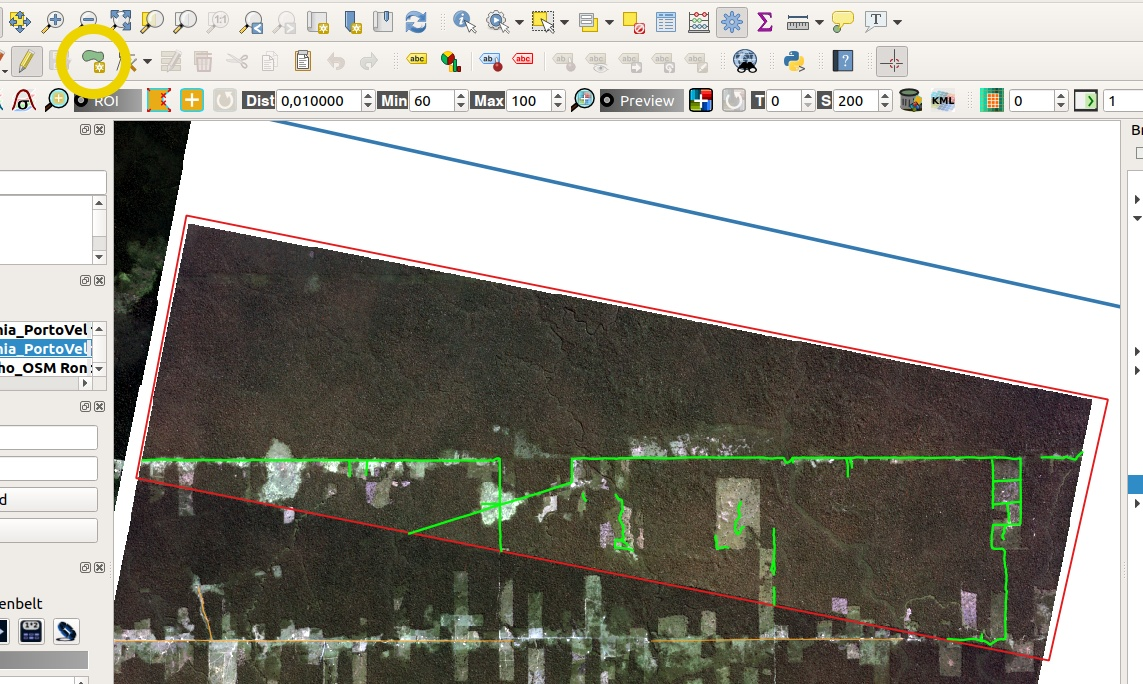
\includegraphics[width=0.9\linewidth]{marking_subAOI01.jpg}
	\caption{Example of a completely labeled satellite image. Manual road labels are in green, the subAOI is the red rectangle. The button for creating polygons like the red subAOI is marked by a yellow circle. At this stage, the labels and satellite image could be 'checked out' and used for generating satellite image tiles for training. Note that below the labeled image there is a further image with only uncorrected OSM labels (orange) which would be next in line for labeling.}
	\label{fig:subaoi}
\end{figure}

\subsection{Labeling roads}
Create a new layer in which the labels will be stored:
\begin{itemize}
	\item Click on the \textit{Layer} Menu Item - \textit{Create Layer} - \textit{New Shape File Layer}
	\item To the right of the edit field for the file name, click on the three dots to select a directory in which to save the data (otherwise QGIS may select your home directory and you may have trouble finding the file). As filename set <AOI>\_roadlabels
	\item Change the file encoding at UTF8 if it is not.
	\item Change the geometry type to \textbf{Line}
	\item Be sure to keep the coordinate system at WGS 84 if not specified otherwise
	\item Add additional field 'label' (integer, 1 digit): this is the type of road (1=paved, 2=unpaved).
	\item Click OK
\end{itemize}

Digitizing:
\begin{itemize}
	\item Be sure to mark the layer just created, because all labeling efforts will apply to the marked layer (marking is done by clicking on the layer in the Layers window). 
	\item Click on the yellow pen symbol in the toolbar. Now the layer editing mode is activated.
	\item Near to the pen symbol, click on the line symbol marked with a little star (a tooltip should pop up if you hover over the icon stating something like: "Add Line Feature").  
	When you now move the cursor to the map section of the screen, the cursor should change to a crosshair.
	\item Now you can start clicking (diligently) along the roads, each point marking a new node of the line. 
	\item To move the map, you can change to the hand tool during digitizing, or you can move across the map with the arrow keys. The middle mouse button will also do the job.
	\item When done with a road or road segment, you can exit digitizing mode with a right mouse click. A window will pop up asking you for the ID and label. Insert a running number for the ID (which is not so important). For label, enter 1 for paved roads (the exception) and 2 if it is an unpaved road or you are not sure (which should be the overwhelming number of cases).
	\item Save the project file in regular intervals (each 10 min or so) in order to prevent inadvertent loss of data
	\item Repeat until all roads in the current subAOI are labeled
	\item Extend the subAOI if you intend to continue labeling, otherwise save the project
\end{itemize}

{\centering\noindent\fbox{
	\parbox{0.85\textwidth}{
		{\fontfamily{pzc}\selectfont {\LARGE With time and patience, the mulberry leaf will become a silk gown.}
		\newline -- Chinese proverb}\newline
		\newline
		As with elaborate garments, patience and conscientious work pay off in road labeling. Please realize that the neuronal networks that will be trained with your labeled data are 'dumb' in the sense that they cannot abstract or infer your intentions; they adhere slavishly to the labels. If you e.g. cut corners, and parts of the resulting label cuts through bushes, the network will be trained to do the same. In other words, incorrect labels are as bad as missing labels. Take your time and 
		\begin{itemize}
			\item choose a zooming level that allows you to place the individual labeling points such that the connecting linear segments are all inside roads, near the centerline
			\item make sure you labeled all roads in a given area that is to be labeled
			\item avoid gaps and overshooting
		\end{itemize}
	The question, then, is how to deal with the various degrees of visibility of small roads. tbc: No clear-cut answer. Extrapolate to some degree. Use GE in case of doubt, but  pay close attention to date: some rural roads vanish/overgrown.
	
	See Figure \ref{fig:label_examples} for orientation.
	}
}
\par
}

\begin{figure}
	\begin{subfigure}{0.48\textwidth}
		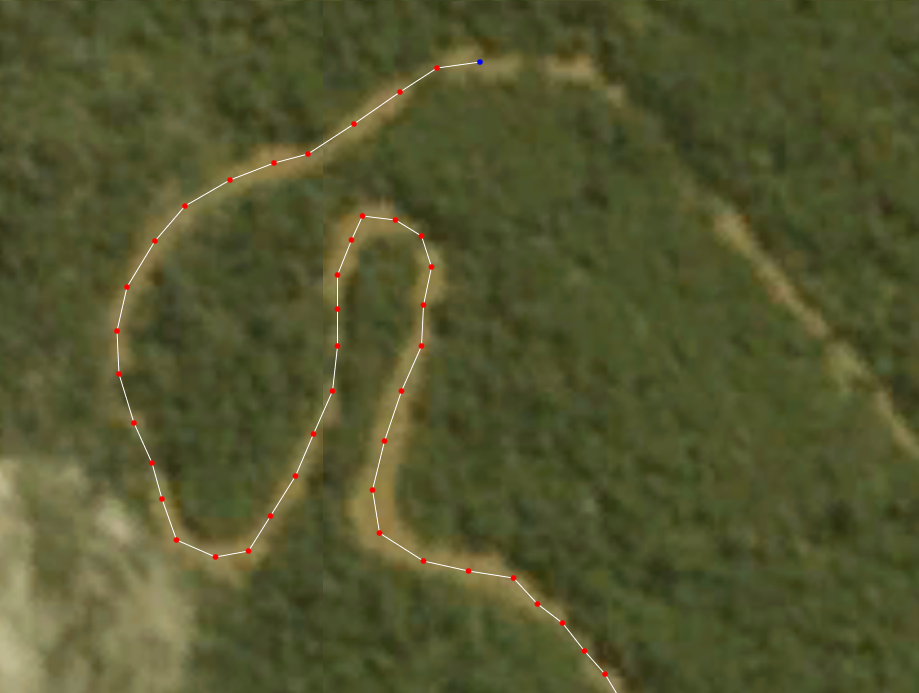
\includegraphics[width=0.957\linewidth]{GE_example_clickclick01_exc.png}
		\label{fig:goodlabel}
	\end{subfigure} 
	\begin{subfigure}{0.48\textwidth}
		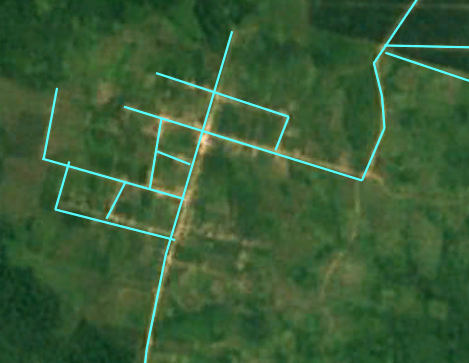
\includegraphics[width=0.957\linewidth]{GE_exemplaryScene_Borneo_allRoads_exc.png}
		\label{fig:badlabel}
	\end{subfigure} 
	\caption{Labeling roads. Left, example of an appropriate level of precision. The image is a screenshot of Google Earth while a small road was in the process of being labeled. Right, example of unacceptable labels. The labels are generally too imprecise; in particular, they are i) partially off-road, ii) incomplete (there are some gaps where roads join each other, and a whole winding road segment is missing in the bottom right quarter), iii) overshooting in some places. Likely, this is a result of labeling at a too zoomed-out level.}
	\label{fig:label_examples}
\end{figure}

\subsubsection{Exporting the data}
When you are done 
\begin{itemize}
	\item Remember: the labels you export must cover satellite images in their entirety. Either a single image or groups of adjacent or overlapping images. Incomplete labels will result in image tiles in which roads exist but are not labeled, downgrading the performance of the Deep Learning Models. 
	\item Therefore, before saving the labels, double-check: do satellite images overlap? If so, have unlabeled parts of an image been overlaid? This can best be checked by temporarily suspending display of all but the labeled images.
	\item Note the file name(s) of the labeled satellite image(s) and pass this information on.
	\item When all's OK, right click on the layer you created
	\item Click  \textit{export} - \textit{Save layer as} - and then choose \textit{Keyhole Markup Language (KML)}. \textbf{Do not choose any other format unless you know exactly how and why!}
	\item Pick a file location and name the file <AOI>\_roadlabels (the extension will be given automatically)
	\item Untick the 'Add saved file to map' box
	\item Leave all other settings
	\item Click OK
	\item Repeat the same procedure (starting with right mouse click - Export...) with the OSM labels of the subAOI (if any). This step needs to be done each time the OSM labels are manipulated in any way. Name the file <AOI>\_OSM
	\item If this is the first time you label roads, verify the correctness of all labels by importing them into Google Earth. This is important, as any basic error will show up here, before you invest many hours of work.
\end{itemize}


\section{Installing and setting up QGIS}
\label{sec:qgis_install}
It is generally recommended to download the Long Term Release (LTR, currently QGIS 3.10.x) of QGIS to avoid any issues. \newline

\textbf{Linux: Installation for Debian/Ubuntu, also tested with Linux Mint 19} \newline
\textit{resource: \url{https://qgis.org/en/site/forusers/alldownloads.html\#debian-ubuntu}} \newline 

It is assumed you have at least rudimentary knowledge of terminal use in Linux. \newline
Otherwise read this: 
\url{https://www.linode.com/docs/tools-reference/tools/using-the-terminal/} \newline
or this: 
\url{https://www.howtogeek.com/140679/beginner-geek-how-to-start-using-the-linux-terminal/} \newline

First, add the QGIS repository to get the newest stable version of QGIS.
This requires to add the qgis.org repository public key to your apt keyring, type:

\begin{verbatim}
wget -O - https://qgis.org/downloads/qgis-2019.gpg.key | gpg --import
gpg --fingerprint 51F523511C7028C3
\end{verbatim}

You can verify the key on this page: \url{https://qgis.org/en/site/forusers/alldownloads.html\#debian-ubuntu}
Now you need to add the key to apt:  

\begin{verbatim}
gpg --export --armor 51F523511C7028C3 | sudo apt-key add -
\end{verbatim}

Next, you have to add specific lines to your /etc/apt/sources.list file.
Be sure to change the version number to your version of Ubuntu or Debian. \newline
This is an example of the entries for the long term release of qgis on Ubuntu 18.04 bionic:

\begin{verbatim}
deb     https://qgis.org/ubuntu-ltr bionic main
deb-src https://qgis.org/ubuntu-ltr bionic main
\end{verbatim}


With the key added to your apt keyring and the repository added to the sources.list file, you can install QGIS and its dependencies:  

\begin{verbatim}
sudo apt-get update
sudo apt-get install qgis python3-qgis qgis-plugin-grass
sudo apt-get install saga
\end{verbatim}

With these steps you should be set up and ready to start with chapter \ref{step2}. \newline

\textbf{MacOS} \newline

To install on MacOS, download the long term release on:
\url{https://qgis.org/en/site/forusers/download.html} and follow the steps described in the installer. Done.\newline

\textbf{Windows} \newline

I recommend using the OSGeo4W network installation method. \newline
The installer can be found here: \url{https://qgis.org/en/site/forusers/download.html} (Download for windows).

OSGeo4W is a package manager allowing you to install the most recent stable versions of QGIS
I will describe the installation process for you here: \newline

\begin{itemize}
	\item When downloaded, open the installer
	\item Select advanced install
	\item Select install from the internet
	\item choose a root directory 
	\item leave the package directory at default
	\item use direct connection if not specified otherwise
	\item (next)
	\item Now there should be a list of Package Repositories
	\item click the "+" next to Desktop
	\item find the package with name "qgis-ltr"
	\item click on the arrow symbol to the left of the row
	\item now it should show a version like 3.4.10 or something
	\item OPTIONAL: 
	\item you can select GRASS GIS and SAGA in the same way (needed for some tools in QGIS)
\end{itemize}

By clicking "next", some dependencies will pop up (just click next and dont change anything in this window).
The dependencies will be downloaded and installed along with qgis.\newline

You are ready to start.

\subsection{Useful windows and features}
\label{subsec:qgis_adjust}
By default QGIS displays just very few panels. There is a multitude of panels with useful features. Those to be displayed can be selected via "View" - "Panels". Their position and arrangement (single vs. in tabs) can be adjusted by standard means (e.g. pulling them with the mouse). The following ones are recommended:
\begin{itemize}
	\item Browser - should show your project folder as "Project Home"  and all the sub-folders and files. May work best on the right side of the screen.
	\item Processing Toolbox
\end{itemize}

Make sure the Digitizing Toolbar is displayed: click on \textit{View} - \textit{Toolbars}, and mark the checkbox \textit{Digitizing Toolbar}.

\subsection{Plugins}
Plugins are a nice way to extend the functionality of QGIS. Navigate to the Plugins Menu, and click on "Manage and Install Plugins" (depending on you internet connection this may take a while to open). In the plugin manager you have the possibility to search, view and install plugins from various sources, including a QGIS plugin repository. 

\subsubsection{The coordinate capture plugin}
\label{coordcap}
This is a useful little tool to quickly extract coordinates from a map canvas. This is a 'core' plugin, so does not need to be installed, but it must be 'activated'. In the Plugin menu's "Installed" tab, tick the according box. Alternatively, navigate to the vectors menu (next to the plugins menu), click on \textit{coordinate capture}. A window will show up (probably docked on the left side of the main window). From there you can click \textit{start capture} and get the coordinates of a clicked point on the screen.



\section{Data: Their types, and how to load them}
This is a short introduction to the data types most common to any GIS.

\subsubsection{Raster data}
\label{rastabands}
Raster Data are discrete, rectangular data matrices.
Each cell of the "Matrix" has a single value and is situated (without any no-data space in between) next to other cells (exept where the borders of the images are of course). \\
Each cell of the raster is also defined by coordinates and a width in X,Y direction (which is the resolution).
An example for raster data are the satellite images you will be labelling. \\

The cell value can be a height, a brightness (0-255) or a color value (either one of red, green and blue).
Rasters of red, green and blue values are combined into RGB images, displaying a color image.  
Cells of the same raster never overlap. \\

\textbf{Excurse: Raster Bands} \newline
Get the semiautomatic classification manual for information about which band contains which wavelength data for 
some of the most widespread satellite platforms: 
\url{https://fromgistors.blogspot.com/p/user-manual.html}\\

You dont need to read the full manual. 
It pays though to have a look at the chapter \textit{Brief introduction to remote sensing}.
There are tables for the image bands of the most common satellite platforms with their ordering of wavelengths/ their names and resolutions.

There is also the combined imagery product specification from planet.com available at: \\
\url{https://www.planet.com/products/planet-imagery/} \\
Scroll down to the button "Download full specs". \\
You are most likely using the Analytic Ortho Scene Product or any other analytic scene.
planet.com did not list their bands according to numbers in the attribute table, i guess the the word order of the band listing seems sufficient to them.
Be sure to check which product you have: 3 or 4 band images (4 band would be better).  
\textit{(Excurse end)}. \\

\textbf{Common file type:} \\

The .tif or .tiff or any .gtiff variation is very common to save raster data, you will most likely work with these file types when you do the labelling job.  

Tiff files can contain multiple bands/ layers of images such as but not limited to the RGB layers of a satellite image,
where each band would correlate to a different sensor of the satellite.
Different satellite platforms have different ways of saving their data: 
The landsat 8 for example does save each of their bands in a separate file while planet.coms ortho analytic scene comes already combined. 

\subsubsection{Vector data}

The most basic Vector Data are Points. The most Basic Attribute vector data can have are coordinates. 
Vector data can have any number of attributes (e.g. temperature, time, concentration, precipitation, average number of people etc. etc. etc.). \\

Next step from points are lines and multi-point lines.
As the smart reader will already have concluded, lines are made of 2 points at least.
We will be creating a lot of line features during the labelling of the satellite images.\\

Another step further down the complexity line are polygons. 
They are made up of a closed multipoint line and generally have a colored filling.
This filling shows an area with an attribute of the same value. \\

\textbf{Common Filetypes:}\\

The esri shape file: .shp. \\
This is a common vector data format, which actually composes of MULTIPLE different files with the same name but different file endings.
If you save vector data to the .shp format you will usually get six files of the same name and different file endings.
When sending these data, it is IMPORTANT to send all the files along with the .shp file. 
Otherwise we will not be able to use the data.\\

google .kml or .kmz files \\
These data formats are quite easy to handle as they are just single files containing all the necessary information.




\end{document}
